% !TEX root = ../main.tex
% SECTION 3: BEANSPRUCHUNGEN (ACHSEN UND WELLEN)
% Inhalt: Liv Erne, Silvio Seiz — Form: ZSF-Template-Rework
% ============================================================

\StartChapter[ch:beanspruchungen]{Beanspruchungen (Achsen und Wellen)}

\SubsectionBar[sec:werkstoffkennwerte]{Werkstoffkennwerte}
\ZSFindex{Werkstoffkennwerte}
\ZSFindex{Spannungs-Dehnungs-Diagramm}

\begin{formulabox}[Spannungs-Dehnungs-Diagramm]
\[ \ZSFstressSigma = \frac{\ZSFstressF}{\ZSFstressAZero} = [\frac{N}{mm^2}] = \ZSFstressE \cdot \ZSFstressEps \qquad \ZSFstressEps = \frac{\ZSFstressDeltaL}{\ZSFstressLZero} \]
\formulanote{$\ZSFstressSigma =$ Spannung, $\ZSFstressEps =$ Dehnung}
\end{formulabox}

% Spalten-Packung (6-Seiten-Ziel): Erklaertext vor die Abbildung gezogen
% (fuellt Spaltenende); Inhalt unverändert.
\begin{runintext}
Manchmal gibt es keine klare \ZSFkeyword{Streckgrenze}, die den linear elastischen Bereich vom plastischen Bereich trennt $\rightarrow \ZSFstressRe \approx \ZSFstressRpZeroTwo$
\end{runintext}

\begin{figbox}[Streckgrenze $\ZSFstressRe$ bzw. $\ZSFstressRpZeroTwo$]
\centering
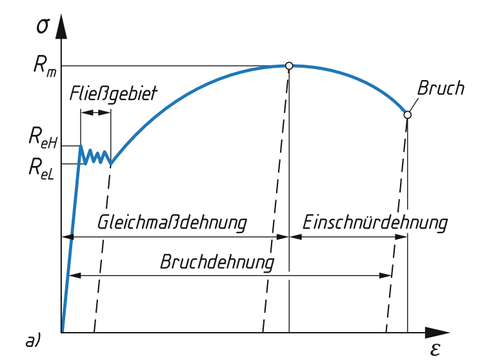
\includegraphics[width=0.40\linewidth,keepaspectratio]{graphics/spannungs_dehnungs_diagramm_streckgrenze_re.png}%
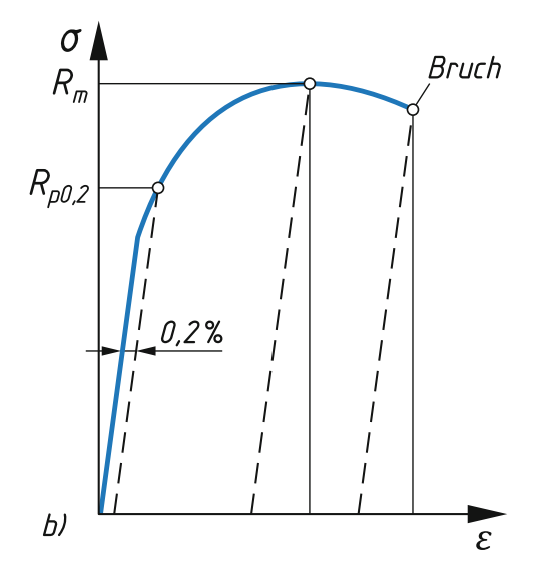
\includegraphics[width=0.30\linewidth,keepaspectratio]{graphics/spannungs_dehnungs_diagramm_dehngrenze_rp02.png}
\end{figbox}
\ZSFindex{Streckgrenze}

\SubsubsectionBar{Werkstofftabelle $\ZSFstressKt = $ Korrekturfaktor}
\ZSFindex{Korrekturfaktor}

\begin{splitbox}[0.51]
\centering
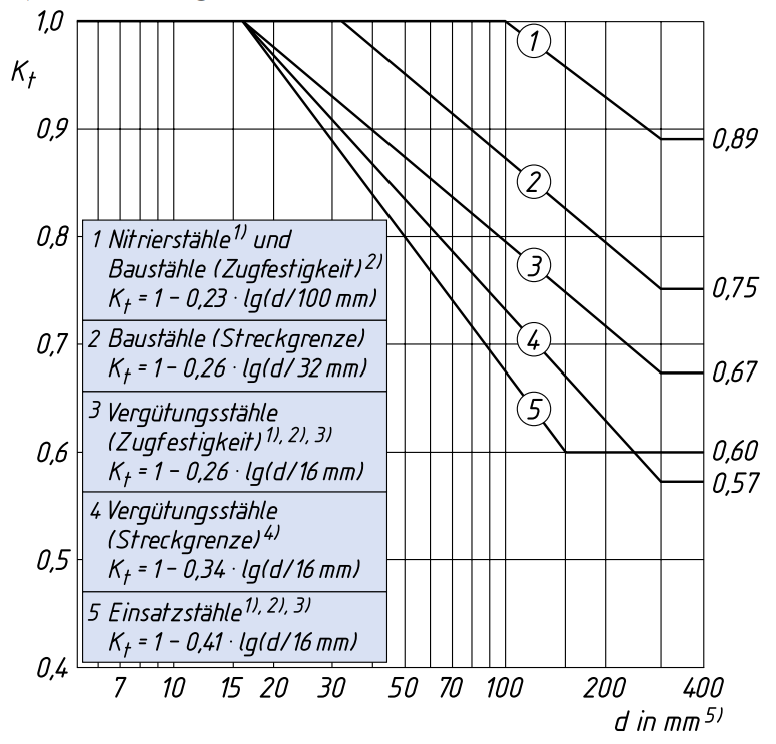
\includegraphics[width=\linewidth,keepaspectratio]{graphics/kt_size_factor_diagram.png}
\tcblower
\ZSFReadableOn
$\ZSFstressKt=1$ bis zu einem\\
bestimmten Durchmesser $\ZSFstressD$,\\
danach $\ZSFstressKt < 1$.
\ZSFgapM

{\centering $\displaystyle \ZSFstressSigmaBW=\ZSFstressKt\cdot\ZSFstressSigmaBWN$\par}
\ZSFgapXS
{\centering $\displaystyle \ZSFstressRe = \ZSFstressKt \cdot \ZSFstressReN$\par}
\ZSFgapXS
{\centering $\displaystyle \ZSFstressRm = \ZSFstressKt \cdot \ZSFstressRmN$\par}
\ZSFgapM

\formulanote{%
  $\ZSFstressSigmaBW$:~Biegewechselfestigkeit\\
  $\ZSFstressRe$:~Streckgrenze\\
  $\ZSFstressRm$:~Zugfestigkeit%
}
\end{splitbox}
\ZSFindex{Biegewechselfestigkeit}
\ZSFindex{Zugfestigkeit}

\SubsectionBar[sec:momente-spannungen]{Momente und Spannungen}

\begin{runintext}
Momente und Spannungen verursacht in Achsen und Wellen durch Zug, Druck, Scherung, Biegung und Torsion.
\end{runintext}

\begin{propertylist}[Belastungsfälle]
\item Konstant
\item Periodisch (Schwellbelastung, Wechselbelastung)
\item Nicht-periodisch
\item Stossartig
\end{propertylist}
\ZSFindex[belastungsfalle]{Belastungsfälle}

\SubsectionBar[sec:sicherheit]{Sicherheit}
\ZSFindex{Sicherheit}

\begin{formulabox}
\[ \frac{Beanspruchbarkeit\ \ZSFstressSafetyR}{Beanspruchung\ \ZSFstressSafetyB} = \frac{ertragbare\ Spannung}{vorhandene\ Spannung} \]
\end{formulabox}

\begin{runintext}
Ideal: $\ZSFstressSafetyR=\ZSFstressSafetyB$ also $\ZSFstressS=1$ \ZSFmuted{$\dots$Sicherheit} $\rightarrow$ Bauteil ist maximal ausgelastet und hält den Belastung stand.
\ZSFdanger{Aber: Keine Reserven für Unsicherheiten} (Gefügefehler, Eigenspannungen, Toleranzen und Fehlbedienungen).
\end{runintext}

\SubsectionBarOnNewColumn[sec:widerstandsmoment]{Widerstandsmoment}
\ZSFindex{Widerstandsmoment}

\begin{tablebox}[Widerstandsmoment $\ZSFstressW$]
\renewcommand{\arraystretch}{1.2}
\begin{ZSFtable}[\ZSFfontTableDense]{Z{1.3} Z{0.925} Z{0.925} Z{0.925} Z{0.925}}
  \ZSFheaderRow
  \ZSFhead{Wellenquerschnitt} & \multicolumn{2}{c}{\ZSFhead{Biegung}} & \multicolumn{2}{c}{\ZSFhead{Torsion}} \\
  \ZSFheaderRow
  & \ZSFhead{$\ZSFstressIb$} & \ZSFhead{$\ZSFstressWb$} & \ZSFhead{$\ZSFstressIt$} & \ZSFhead{$\ZSFstressWt$} \\
  \ZSFtablestrut
  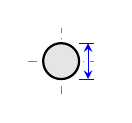
\begin{tikzpicture}[scale=0.38, baseline=-0.12cm]
    \draw[dashdotted, thin, gray] (-1.1,0) -- (1.1,0);
    \draw[dashdotted, thin, gray] (0,-1.1) -- (0,1.1);
    \draw[thick, fill=gray!20] (0,0) circle (0.6);
    \draw[thin, blue] (0.6, 0.6) -- (1.1, 0.6);
    \draw[thin, blue] (0.6, -0.6) -- (1.1, -0.6);
    \draw[<->, >=stealth, thin, blue] (0.9, -0.6) -- (0.9, 0.6) node[midway, right=-1pt] {$\ZSFstressD$};
  \end{tikzpicture}
  & $\frac{\pi}{64} \cdot \ZSFstressD^4$ & $\frac{\pi}{32} \cdot \ZSFstressD^3$ & $\frac{\pi}{32} \cdot \ZSFstressD^4$ & $\frac{\pi}{16} \cdot \ZSFstressD^3$ \\
  \ZSFtablestrut
  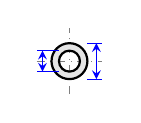
\begin{tikzpicture}[scale=0.38, baseline=-0.12cm]
    \draw[dashdotted, thin, gray] (-1.1,0) -- (1.1,0);
    \draw[dashdotted, thin, gray] (0,-1.1) -- (0,1.1);
    \draw[thick, fill=gray!20, even odd rule] (0,0) circle (0.6) (0,0) circle (0.35);
    % d on the left
    \draw[thin, blue] (-0.35, 0.35) -- (-1.1, 0.35);
    \draw[thin, blue] (-0.35, -0.35) -- (-1.1, -0.35);
    \draw[<->, >=stealth, thin, blue] (-0.9, -0.35) -- (-0.9, 0.35) node[midway, left=-1.5pt] {$\ZSFstressD$};
    % D on the right
    \draw[thin, blue] (0.6, 0.6) -- (1.1, 0.6);
    \draw[thin, blue] (0.6, -0.6) -- (1.1, -0.6);
    \draw[<->, >=stealth, thin, blue] (0.9, -0.6) -- (0.9, 0.6) node[midway, right=-1pt] {$\ZSFstressDbig$};
  \end{tikzpicture}
  & $\frac{\pi}{64} \cdot (\ZSFstressDbig^4 - \ZSFstressD^4)$ & $\frac{\pi}{32} \cdot \frac{\ZSFstressDbig^4 - \ZSFstressD^4}{\ZSFstressDbig}$ & $\frac{\pi}{32} \cdot (\ZSFstressDbig^4 - \ZSFstressD^4)$ & $\frac{\pi}{16} \cdot \frac{\ZSFstressDbig^4 - \ZSFstressD^4}{\ZSFstressDbig}$ \\
\end{ZSFtable}
\formulanote{$\ZSFstressW = \ZSFstressI / e_{\max} =$ Widerstand gegen Randfaser-Spannung, $\ZSFstressI =$ geom.\ Widerstand gegen Verformung (Biegung/Torsion)}
\end{tablebox}

\SubsectionBar[sec:biegung]{Biegemoment $\ZSFstressMb$ und -Spannung $\ZSFstressSigmaB$}
\ZSFindex{Biegemoment}
\ZSFindex{Biegespannung}

\begin{runintext}
Durch Normalspannung verursacht (Zug/ Druck \ZSFref{sec:momverlaeufe}).
\end{runintext}

\begin{formulabox}
\formulasources{$\ZSFstressWb$:~\ZSFsource{bestimmen mit}{sec:widerstandsmoment} \ $\cdot$ \ Momentenverlauf: \ZSFsource{bestimmen mit}{sec:momverlaeufe}}
\[ \ZSFstressMb = \ZSFstressF \cdot \ZSFstressApos \qquad \ZSFstressSigmaB = \frac{\ZSFstressMb}{\ZSFstressWb} \]
\[ \ZSFstressSigmaB = \frac{32 \cdot \ZSFstressMb}{\pi \cdot \ZSFstressD^3} \]
\formulanote{$\ZSFstressApos$:~Hebelarm bzw. Position der Kraft ab Lager A}
\formulanoteabove{Max.\ Biegemoment bei 2 Lagern (Kraft bei $\ZSFstressApos$):}
\[ \ZSFstressMbMax = \frac{\ZSFstressApos\,(\ZSFstressL-\ZSFstressApos)}{\ZSFstressL}\cdot\sqrt{\ZSFstressFt^2 + \ZSFstressFr^2} \]
\ZSFgapXS
\centering
\begin{tikzpicture}[x=1pt, y=1pt, >=latex, font=\sffamily\fontsize{5.5}{6.5}\selectfont]
  \def\wL{115}
  \def\aPos{42}
  \def\leftS{8}
  \def\rightS{107}

  % Hilfslinien fuer Bemassung (sehr duenn, grau)
  \draw[ultra thin, gray, dashed] (\leftS, 6) -- (\leftS, -26);
  \draw[ultra thin, gray, dashed] (\aPos, 6) -- (\aPos, -26);
  \draw[ultra thin, gray, dashed] (\rightS, 6) -- (\rightS, -26);

  % 1. Biegemomentenverlauf
  % Momenten-Flaeche
  \fill[fill=\chaptercolorlight!40] (\leftS, -3) -- (\aPos, -10) -- (\rightS, -3) -- cycle;
  % Null-Linie
  \draw[thick, gray] (\leftS, -3) -- (\rightS, -3);
  % Verlauf
  \draw[very thick, \chaptercolor] (\leftS, -3) -- (\aPos, -10) -- (\rightS, -3);
  % Beschriftung Momentenverlauf
  \node[right, \chaptercolor, font=\sffamily\fontsize{4}{5}\selectfont] at (\rightS-22, -6.5) {$\ZSFstressMb(x)$};
  \node[below, \chaptercolor, inner sep=0.5pt, font=\sffamily\fontsize{4.5}{5.5}\selectfont] at (\aPos, -10) {$\ZSFstressMbMax$};

  % 2. Traeger (Welle)
  \draw[thick, fill=black!5] (\leftS, 6) rectangle (\rightS, 9);
  \draw[densely dashed, gray] (\leftS, 7.5) -- (\rightS, 7.5);

  % Lager A (Festlager)
  \draw[thick] (\leftS, 6) -- (\leftS, 4.5);
  \draw[thick, fill=white] (\leftS, 4.5) -- (\leftS-2.5, 0.5) -- (\leftS+2.5, 0.5) -- cycle;
  \draw[thick] (\leftS-3.5, 0.5) -- (\leftS+3.5, 0.5);
  \foreach \xx in {-2.5,-0.5,1.5}
    \draw (\leftS+\xx, 0.5) -- (\leftS+\xx-0.8, -1);
  \node[left, inner sep=0.5pt] at (\leftS-3.5, 2.5) {\scriptsize A};

  % Lager B (Loslager)
  \draw[thick] (\rightS, 6) -- (\rightS, 4.5);
  \draw[thick, fill=white] (\rightS, 4.5) -- (\rightS-2.5, 0.5) -- (\rightS+2.5, 0.5) -- cycle;
  \fill (\rightS-1.2, -0.8) circle (0.5);
  \fill (\rightS+1.2, -0.8) circle (0.5);
  \draw[thick] (\rightS-3.5, -1.8) -- (\rightS+3.5, -1.8);
  \node[right, inner sep=0.5pt] at (\rightS+3.5, 2.5) {\scriptsize B};

  % Kraft F_res (zeigt nach unten)
  \draw[->, very thick, \chaptercolor] (\aPos, 18) -- (\aPos, 10);
  \node[above, inner sep=0.5pt] at (\aPos, 17) {$\sqrt{\ZSFstressFt^2\!+\!\ZSFstressFr^2}$};

  % 3. Bemassung
  % a und L-a
  \draw[|<->|] (\leftS, -18) -- node[fill=white, inner sep=0.6pt] {$\ZSFstressApos$} (\aPos, -18);
  \draw[|<->|] (\aPos, -18) -- node[fill=white, inner sep=0.6pt] {$\ZSFstressL\!-\!\ZSFstressApos$} (\rightS, -18);
  % L darunter
  \draw[|<->|] (\leftS, -24) -- node[fill=white, inner sep=0.6pt] {$\ZSFstressL$} (\rightS, -24);
\end{tikzpicture}
\end{formulabox}

\SubsectionBar[sec:torsion]{Torsionsmoment $\ZSFstressMt$ und -Spannung $\ZSFstressTauT$}
\ZSFindex{Torsionsmoment}
\ZSFindex{Torsionsspannung}

\begin{runintext}
Durch Schubspannungen verursacht (Verschiebung).
\end{runintext}

\begin{splitbox}[0.57][sidebyside align=center]
\formulasources{$\ZSFstressWt$:~\ZSFsource{bestimmen mit}{sec:widerstandsmoment}}
{\centering $\displaystyle \ZSFstressMt = \ZSFstressF \cdot \ZSFstressR \qquad \ZSFstressTauT = \frac{\ZSFstressMt}{\ZSFstressWt}$\par}
\ZSFgapS
{\centering kreisförmiger Vollquerschnitt:\par}
\ZSFgapS
{\centering $\displaystyle \ZSFstressTauT = \frac{16 \cdot \ZSFstressMt}{\pi \cdot \ZSFstressD^3}$\par}
\tcblower
\centering
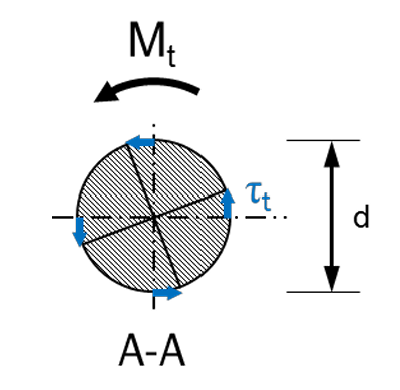
\includegraphics[width=0.6\linewidth,keepaspectratio]{graphics/v5_torsionsspannung_welle.png}
\end{splitbox}

\begin{formulabox}[Zulässige Torsionsspannung $\ZSFstressTauTzul$]
\[ \ZSFstressDmin = \sqrt[3]{\frac{16\cdot \ZSFstressMt}{\pi \cdot \ZSFstressTauTzul}} \qquad \ZSFstressTauTzul = \frac{16\cdot \ZSFstressMt}{\pi \cdot \ZSFstressDmin^3} = \frac{\ZSFstressTauTWN}{\ZSFstressSD} \]
\formulanote{\ZSFReadableOn mit Torsionswechselfestigkeit $\ZSFstressTauTWN$ und Sicherheit gegen Dauerbruch $\ZSFstressSD$}
\end{formulabox}

\begin{valuegridcustom}{l X[l]}[$\ZSFstressSD$]
\textbf{3} & Kurze und dünne Welle, keine Kerben, keine Stösse \\
\textbf{4} & Lange und dicke Welle, viele Kerben, starke Stösse
\end{valuegridcustom}

\SubsectionBar[sec:vergleichsspannung]{Vergleichsspannung $\ZSFstressSigmaV$}
\ZSFindex{Vergleichsspannung}

\begin{runintext}
Bei Kombination von Torsion und Biegung \ZSFref{sec:momverlaeufe}. Damit die Welle nicht zerbricht:
\end{runintext}

\begin{formulabox}
\formulasources{$\ZSFstressSigmaB$:~\ZSFsource{aus}{sec:biegung} \ $\cdot$ \ $\ZSFstressTauT$:~\ZSFsource{aus}{sec:torsion}}
\[ \ZSFstressSigmaV = \sqrt{\ZSFstressSigma^2 + 3\cdot   \ZSFstressTau^2} \qquad \ZSFstressSigmaV < \ZSFstressSigmaBWN \]
\[ \ZSFstressSigma= \ZSFstressSigmaRes = \ZSFstressSigmaZd + \ZSFstressSigmaB \qquad \ZSFstressTau = \ZSFstressTauRes = \ZSFstressTauS + \ZSFstressTauT \]
\formulanote{$\ZSFstressSigmaZd$:~Zug-/Druckspannung \ $\cdot$ \ $\ZSFstressTauS$:~Scherspannung}
\end{formulabox}

%\ZSFmuted{
%Schubspannungshypothese: $\sigma_v = \sqrt{\sigma^2 + 4\cdot   \tau^2}$
%Normalspannungshypothese: $\sigma_v = 0.5 \cdot (\sigma+ \sqrt{\sigma^2 + 4\cdot   \tau^2})$
%}
%\ZSFfig{graphics/vergleichsspannung_entscheidungsbaum.png}{Vergleichsspannung}{}

\SubsectionBar[sec:kerben]{Kerben}
\ZSFindex{Kerbe}
\ZSFindex{Kerbformzahl}

\begin{runintext}
\ZSFkeyword[Kerbe]{Kerben} sind kritische Stellen, da sie hohe Momente bei kleinen Durchmessern übertragen (Mehraxialer Spannungszustand im Kerbbereich).
\end{runintext}

\begin{formulabox}
\[ \ZSFstressSigmaMax = \ZSFstressAlphaK \cdot \ZSFstressSigmaN \qquad \ZSFstressTauTMax = \ZSFstressAlphaK \cdot \ZSFstressTauN \]
\[ \ZSFstressT = \frac{\ZSFstressDbig - \ZSFstressD}{2} \]
\formulanote{$\ZSFstressAlphaK$:~Kerbformzahl \ $\cdot$ \ $\ZSFstressSigmaN$, $\ZSFstressTauN$:~Nennspannung \ $\cdot$ \ $\ZSFstressT$:~Nuttiefe}
\end{formulabox}

\begin{figbox}[Kraftverteilung an Kerben]
  \centering
  $\vcenter{\hbox{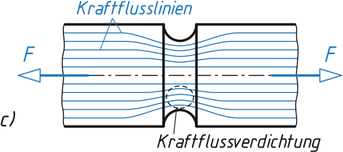
\includegraphics[width=0.25\linewidth,keepaspectratio]{graphics/kerben_split/c.png}}}$\hfill
  $\vcenter{\hbox{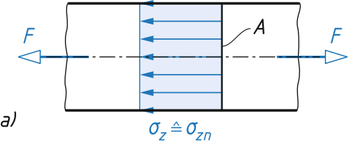
\includegraphics[width=0.25\linewidth,keepaspectratio]{graphics/kerben_split/a.png}}}$\hfill
  $\vcenter{\hbox{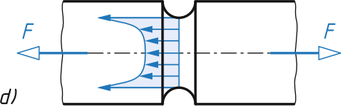
\includegraphics[width=0.25\linewidth,keepaspectratio]{graphics/kerben_split/d.png}}}$\par\ZSFgapXS
  $\vcenter{\hbox{\phantom{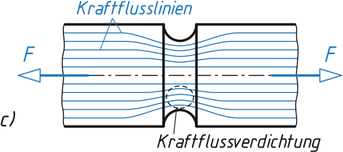
\includegraphics[width=0.25\linewidth,keepaspectratio]{graphics/kerben_split/c.png}}}}$\hfill
  $\vcenter{\hbox{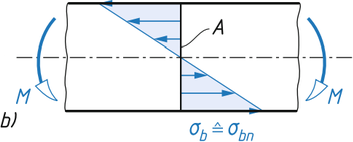
\includegraphics[width=0.25\linewidth,keepaspectratio]{graphics/kerben_split/b.png}}}$\hfill
  $\vcenter{\hbox{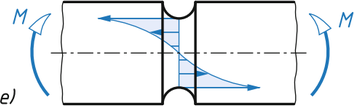
\includegraphics[width=0.25\linewidth,keepaspectratio]{graphics/kerben_split/e.png}}}$
\end{figbox}
